\documentclass[12pt]{article}
\usepackage[pdftex]{graphicx}
% and their extensions so you won't have to specify these with
% every instance of \includegraphics
\DeclareGraphicsExtensions{.pdf,.jpeg,.png}
\usepackage{url}

\newcommand{\psykal}{{PS}y{KA}l}

\begin{document}

\title{Analysing the Performance of Shallow-Water Models with the
 Roofline Model}

\author{A.~.R.~Porter and R.~W.~Ford}

\maketitle

\section{Introduction}

We want to use the Roofline Model to establish the efficiency (or
otherwise) of two shallow-water benchmark codes that we have used in
the GOcean project. The first of these codes, Shallow, was originally
written by Paul Swarztrauber over 30 years ago and has been optimised
by various people over that time. In contrast, nemolite2d is a new,
un-optimised code that has been extracted from NEMO.

Although we have investigated how the performance of the \psykal
version of nemolite2d compares with that of the original, we have not
addressed how efficient the original actually is. In order to do so we
use the Roofline Model~\cite{roofline} which provides a relatively
simple way of characterising the performance of a code in terms of
whether it is memory-bandwidth bound or compute bound.

In this report we investigate the application of the Roofline Model to
these two, serial, shallow-water codes.

\section{Hardware Details}

We have performed this investigation on two different Intel CPUs; an
E5-1620 v.2 and an E5-2697 v.2. Both of these use the Intel Ivy Bridge
microarchitecture and have Ivy Bridge-EP cores. More details are given
in Table~\ref{TAB_stream_linpack}.

\begin{table}
\begin{tabular}{|l|c|c|c|c|}
\hline
  \multicolumn{5}{|c|}{E5-1620 v.~2, 3.7GHz} \\
  \hline
LINPACK (GFLOPS) & \multicolumn{4}{c|}{28.32} \\
\hline
&  L1 Cache & L2 Cache & L3 Cache & Main memory \\
$n$-way set associative & 8    & 8   & 10 & -- \\
Size                  &   32 KB/core   & 256 KB/core   & 10 MB    &  -- \\
\hline
STREAM2 (GB/s)   &  160  &  61.0  & 46.0 &  20.5 \\
  \hline
\multicolumn{5}{|c|}{E5-2697 v.~2, 2.7GHz}  \\
\hline
LINPACK (GFLOPS) & \multicolumn{4}{c|}{25.41} \\
\hline
               & L1 Cache & L2 Cache & L3 Cache & Main memory \\
$n$-way set associative & 8    & 8   & 20 & -- \\
Size           &   32 KB/core  & 256 KB/core   & 30 MB    &  -- \\
\hline
STREAM2 (GB/s) & 132      & 59.0     & 40.0     &  20.2 \\
\hline
\end{tabular}
\caption{The STREAM2 (DAXPY) and LINPACK benchmark results for a
  single thread running on each of the two CPUs considered here.}
\label{TAB_stream_linpack}
\end{table}

In applying the roofline model we follow the approach suggested
in~\cite{para_pearls} and use the well-known STREAM~\cite{stream} and
LINPACK~\cite{linpack} benchmarks in order to get the upper bounds on
the memory bandwidth and FLOPS for the test hardware. Since we are
using Intel CPUs we used the Intel Math Kernel Library implementation
of LINPACK.

Interpreting the results of the STREAM benchmark in order to get
bandwidth figures for all levels of the cache hierarchy is not
straightforward. We therefore used the STREAM2 benchmark which is
intended for this purpose. In Figure~\ref{FIG_stream2} we plot the
results obtained from the DAXPY component of the STREAM2 benchmark on
the E5-2697 CPU (using v.~14 {\bf (check this)} of the Intel
compiler. The plateaux in bandwidth for L2, L3 and main memory are
clear but that for L1 is considerably noisier. The final values we
have used in the roofline plots are given in
Table~\ref{TAB_stream_linpack}.

\begin{figure}
\includegraphics[width=120mm]{stream2_archer}
\caption{Results from running the STREAM2 benchmark on the E5-2697
  CPUs. Error bars indicate the maximum and minimum values obtained
  from 200 repeats of each case.  size. }
\label{FIG_stream2}
\end{figure}

 The equivalent results for the E5-1620 CPU are shown in
 Figure~\ref{FIG_daxpy_bw}. This plot has the same shape as that for
 the E5-2697 but is shifted upwards indicating an increase in
 bandwidth accross all levels of the cache hierarchy, but particularly
 for L3 and L1. In addition, the width of the plateau corresponding to
 the L3 cache is narrower because of the smaller size of this cache on
 the E5-1620.

\begin{figure}
\includegraphics[width=120mm]{daxpy_bw_perf}
\caption{Bandwidth obtained on the E5-1620 CPU by the original and
  modified versions of the daxpy kernel from the STREAM2 benchmark.}
\label{FIG_daxpy_bw}
\end{figure}

\section{Hardware Performance Counters}

Initially, we hoped to use Hardware Performance Counters (HWPCs) in
order to get an accurate measure of the FLOPS and memory traffic
associated with specific kernels in each of the models.

The likwid tool (\url{https://github.com/RRZE-HPC/likwid}) gives
access to HWPCs on Intel and AMD CPUs.
However, there are issues with the accuracy of these counters,
especially for FLOP-related measurements on Ivy Bridge architectures. A
tool is included in the likwid distribution that tests the accuracy of
HWPC-derived data by running micro-benchmarks for which the FLOP count
and memory traffic are known:
\url{https://code.google.com/p/likwid/wiki/IvyBridgeVerification}.
The results of doing this on an Intel Xeon E5-1620 v2 CPU are shown in
Figure~\ref{FIG_flops_dp_test}. It appears that once the memory
footprint spills out of L1 cache (which all of our nemolite2d
benchmark configurations do), the performance counter results
significantly overestimate the FLOPs performed.

\begin{figure}
\centering
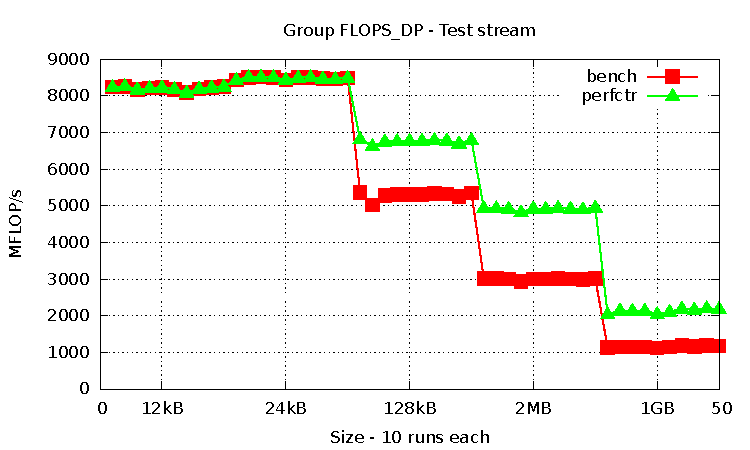
\includegraphics[width=120mm]{FLOPS_DP_stream_ivybridgeEP.pdf}
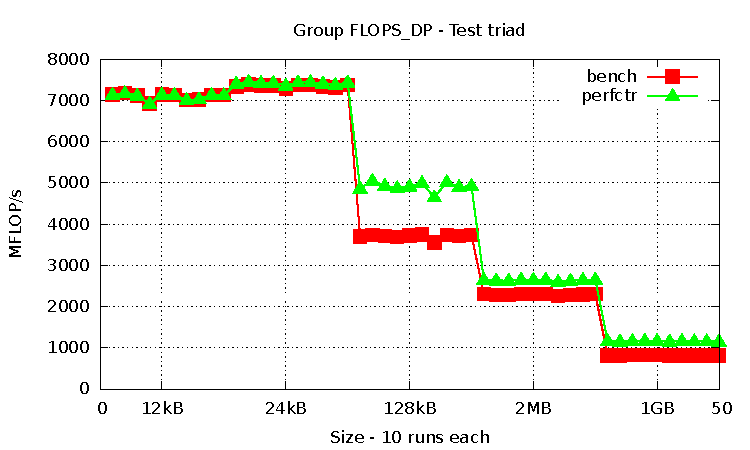
\includegraphics[width=120mm]{FLOPS_DP_triad_ivybridgeEP.pdf}
\caption{Results of the likwid accuracy test for the FLOPS\_DP group
  and the stream (top) and triad (bottom) benchmark on an Intel Xeon
  E5-1620 v2.}
\label{FIG_flops_dp_test}
\end{figure}

We therefore need some other way of measuring FLOPS. We could use
likwid on an older Intel CPU (to which we have root access) or try
another tool on the IvybridgeEP system. Other possible tools include
Intel's VTune or OProfile.

Despite the unreliability of the absolute values of the FLOP counts,
we hope that the trends in HWPC data as the problem size is varied
will be useful. This raw data is given in Table~\ref{TAB_hwpc_mom_u}.

\begin{table}
\begin{tabular}{l|l|l|l|l}
\hline
\hline
               & \multicolumn{4}{c}{Problem size} \\
               & 32     &    64        &    128       &   256 \\
\hline
Footprint (MB) & 0.1 & 0.5          & 2.3          & 9.2 \\
\hline
Runtime (RDTSC) [s]   & 0.144868 &  0.4485108   &   1.697142   &   6.446171  \\
Runtime unhalted [s]  & 1.199456e-01 & 4.475135e-01 & 1.750448e+00 &   6.734944e+00 \\
CPI                   & 6.431867e-01 & 6.423220e-01 & 6.503796e-01 &   6.348858e-01 \\
\hline
MFLOPS           & 3.112780e+03 & 3.877720e+03  & 4.163209e+03 & 4.304728e+03 \\
AVX MFLOPS       & 2.840625e+03 & 3.660086e+03  & 3.993397e+03 & 4.164647e+03 \\
Packed MUOPS/s   & 7.423377e+02 & 9.584935e+02  & 1.046781e+03 & 1.092280e+03 \\
Scalar MUOPS/s   & 2.077927e+02 & 1.306897e+02  & 7.294811e+01 & 3.784506e+01 \\
\hline
L1 DTLB load misses          &      2007     &      17015   &    1317912   &    6748712   \\
L1 DTLB load miss rate       &  2.949686e-06 &  6.607264e-06& 1.326630e-04 & 1.723565e-04 \\
L1 DTLB load miss durn [Cyc] &  3.970154e+01 &  3.080153e+01& 2.101039e+01 & 2.013584e+01 \\
L1 DTLB store misses         &       77      &       16     &     87257    &    401036    \\
L1 DTLB store miss rate      &  1.131668e-07 &  6.213119e-09& 8.783423e-06 & 1.024213e-05 \\
L1 DTLB store miss durn [Cyc]&  5.633766e+01 &       29     & 2.151055e+01 & 2.669793e+01 \\
\hline
L2D load bandwidth [MB/s]  &  3.811099e+03 &  5.030691e+03 & 1.080936e+04 & 1.446214e+04 \\
L2D load data volume [GB]  &   0.541220288 &   2.34655488  &  18.1215488  &   92.177536  \\
L2D evict bandwidth [MB/s] &  3.131102e+02 &  3.094459e+02 & 4.501487e+02 & 5.065637e+02 \\
L2D evict data volume [GB] &   0.04446528  &   0.144340352 &  0.75465984  &  3.22869248  \\
L2 bandwidth [MB/s]        &  4.600834e+03 &  5.493404e+03 & 1.130282e+04 & 1.498363e+04 \\
L2 data volume [GB]        &   0.653371776 &   2.562386304 & 18.948807808 & 95.501414592 \\
\hline
L3 load bandwidth [MB/s]  &  2.434255e+03 & 4.626177e+03 & 4.511686e+03 & 4.607617e+03 \\
L3 load data volume [GB]  &   0.371968512 &  2.07489024  &   7.6168768  &   29.692832  \\
L3 evict bandwidth [MB/s] &  5.652167e+02 & 4.828169e+02 & 2.771148e+02 & 2.722823e+02 \\
L3 evict data volume [GB] &   0.086368448 &  0.216548608 &  0.467840512 &  1.75466688  \\
L3 bandwidth [MB/s]       &  2.999472e+03 & 5.108994e+03 & 4.788801e+03 & 4.879899e+03 \\
L3 data volume [GB]       &   0.45833696  &  2.291438848 &  8.084717312 &  31.44749888 \\
\hline
\hline
\end{tabular}
\caption{Hardware performance counter data obtained using the likwid
  tool for the u-Momentum kernel on the Intel E5-1620 v2 processor.}
\label{TAB_hwpc_mom_u}
\end{table}

\section{Performance Analysis with the Roofline Model}

\subsection{Calculating Kernel Characteristics}

Although the Continuity kernel is very simple, the u-Momentum kernel
is not and in particular, includes a call to the {\tt sin()} function.
In order to estimate the cost of this function in FLOPs, the following
code was compiled (with the Intel compiler and -O1) and run with
likwid-perfctr:
\begin{verbatim}
  my_sum = 0.0d0
  do i = 1, 1000
    my_sum = my_sum + sin(real(i))
  end do
  write (*,*) 'My sum = ', my_sum
\end{verbatim}
This measurement revealed that the {\tt sin()} function requires
approximately 13 FLOPs.

A key component of the Roofline model is the Arithmetic Intensity of
the code being executed:
\begin{equation}
AI = \frac{\textrm{No. of floating-point operations}}{\textrm{Bytes fetched from memory}}
\end{equation}
Since HWPC data proved to be unreliable, we calculated this quantity
manually by examining the source code and counting the number of
memory references and arithmetic operations that it contained. In
doing this counting we assume that any references to adjacent array
elements are fetched in a single cache-line and thus only count once.

To illustrate this, we consider the first loop-nest in the
time-stepping section of the Shallow code. This is a doubly-nested
loop over {\tt i} and {\tt j} with {\tt i} innermost. The body of the
loop is:
\begin{verbatim}
CU(I+1,J) = .5d0*(P(I+1,J)+P(I,J))*U(I+1,J)
CV(I,J+1) = .5d0*(P(I,J+1)+P(I,J))*V(I,J+1)
Z(I+1,J+1) =(FSDX*(V(I+1,J+1)-V(I,J+1))- &
             FSDY*(U(I+1,J+1)-U(I+1,J)))/&
            (P(I,J)+P(I+1,J)+            &
             P(I+1,J+1)+P(I,J+1))
H(I,J) = P(I,J)+0.25d0*                   &
         (U(I+1,J)*U(I+1,J)+U(I,J)*U(I,J) & 
         +V(I,J+1)*V(I,J+1)+V(I,J)*V(I,J))
\end{verbatim}
This code writes to four memory locations ({\tt CU}, {\tt CV}, {\tt Z}
and {\tt H}) and reads from ten distinct locations.  However, if we
assume caching of reads from locations adjacent in memory ({\it e.g.} {\tt
  P(i,j)} and {\tt P(i+1,j)}) then we have only six distinct reads.
If we assume that each of these ten memory accesses will touch a
separate cache line then this code fragment will result in the moving
of ten cache lines, each of which is 64 bytes (eight double-precision
words). However, as noted above, this code fragment is the body of a
loop nest. Therefore, upon the next loop trip, {\tt i} will have been
incremented by one and the majority of the accessed values will still
be in cache. In fact, a new cache line will only have to be fetched
every seven trips of the (innermost) loop and thus the mean memory
traffic per loop trip is approximately $640/7$ bytes.

We can also count the number of floating-point arithmetic operations
(FLOPs) in this code fragment which gives us 12 multiplications and 12
additions. The $AI$ for this code fragment is then $24*7/640 = 0.26$
FLOPs/byte.  If we do the same analysis for the (longer) u-Momentum
kernel of nemolite2d then we find that there are 51 addition
operations, 56 multiplication/division operations and one call to {\tt
  sin()}. There are 31 distinct memory references. This gives an $AI$
of approximately $(107+13)*7/(31*64) = 0.42$ FLOPs/byte (where we
assume the call to {\tt sin()} costs 13 FLOPs). The results of this
analysis are summarised in Table~\ref{TAB_kernel_details}.

\begin{table}
\begin{tabular}{|l|c|c|c|}
\hline
Code                       & Shallow & \multicolumn{2}{c|}{nemolite2d} \\
\hline
Kernel                     & 1st loop nest & Continuity & u-Momentum \\
\hline                                
FLOPs                      & 24      &    14      &   107+13   \\
Distinct memory refs       & 10      &    10      &   31       \\
$AI$ (FLOPs/byte)          & 0.26    &  0.153     &   0.42     \\
Working-set size (bytes)   & $56n^2$ &  $64n^2$   &   $136n^2$ \\
\hline
\end{tabular}
\caption{Details of the kernels investigated with the roofline
  model. $n$ is the problem size -- the length of one side of the
  square domain.}
\label{TAB_kernel_details}
\end{table}

We measure the mean time to execute the u-Momentum kernel over the
whole domain as 0.0021 seconds (Intel v.16 on the E5-1620) for the
$256^2$ problem size. This gives us a performance of $\frac{120\times
  256^2}{0.0021} = 3.7$ GFLOPS. (In contrast, instrumenting this
section of code with the LIKWID marker API and using likwid-perfctr we
measure 4.7 GFLOPS.)  For the $128^2$ domain, the measured time is
0.556E-03 s. This gives a performance of $\frac{120\times
  128^2}{0.556\times10^{-3}} = 3.5$ GFLOPS which again is some 25\% less
than we measure directly with likwid.

Using these figures we can finally construct the Roofline model for
the two CPUs and the various kernels. In
Figure~\ref{FIG_roofline_archer} we plot the model for the E5-2697 CPU
and show the performance of the 1st loop-nest of Shallow and the
u-Momentum kernel of nemolite2d. Two things are immediately clear from
this plot: first, the performance of the first loop nest of Shallow is
clearly memory-bandwidth limited and second, the u-Momentum kernel of
NEMOLite2D is no-where near approaching this limit.

\begin{figure}
\centering
\includegraphics[width=120mm]{roofline_archer}
\caption{Comparison of the performance achieved by NEMOLite2D and
  Shallow on the E5-2697 CPU.}
\label{FIG_roofline_archer}
\end{figure}

Two performance points are plotted for the Shallow kernel
corresponding to domains of $512^2$ and $1024^2$. Using the equation
for working-set size in Table~\ref{TAB_kernel_details}, these
correspond to 14.7 and 58.7~MB, respectively. Since the E5-2697 has
an L3 cache of 30~MB, the $512^2$ case should be contained in cache
while the $1024^2$ case will spill to main memory. This is borne out
by the plot; the $1024^2$ case is achieving a performance in-line
with saturating the bandwidth to main memory. The $512^2$ case is
approaching the L3 bandwidth limit. We investigate the reasons for
the fact that it does not achieve the L3 bandwidth limit below.
 
In contrast to the results obtained with the Shallow kernel, the
performance of the NEMOLite2D u-Momentum kernel shows little
sensitivity to working-set size -- the $128^2$, $256^2$ and $512^2$
performance points in Figure~\ref{FIG_roofline_archer} are very close
together.

In Figure~\ref{FIG_roofline_haswell} we plot the Roofline model
obtained for the E5-1620 CPU. In order to investigate the poor
performance of the u-Momentum kernel of NEMOLite2D, we also show the
performance of the (simpler) Continuity kernel from that code. As we
would expect, the performance of the u-Momentum kernel remains poor on
this CPU. For the $512^2$ domain the Continuity kernel performs well,
reaching the limit imposed by the bandwidth to main memory. However,
the working-set sizes for this kernel for the $128^2$ and $256^2$
domains are approximately 1~MB and 4.2~MB, respectively and therefore
both of these should fit comfortably within L3 cache. Despite this,
the performance achieved with these domain sizes falls short of the L3
bandwidth limit.  Although this kernel is one of several within the
time-stepping loop of NEMOLite2D, the working-set size of this loop
for the $128^2$ domain is just 2.4~MB which again is well within the
capacity of L3.

\begin{figure}
\centering
\includegraphics[width=120mm]{roofline_haswell}
\caption{Comparison of the performance achieved by different
  NEMOLite2D kernels on the E5-1620 CPU.}
\label{FIG_roofline_haswell}
\end{figure}

In order to investigate why the performance of the Continuity kernel
is falling well short of the maximum predicted by the roofline model
we have experimented with the level of SIMD
vectorisation. Figure~\ref{FIG_kernel_perf} shows the performance of
the Continuity and u-Momentum kernels when compiled without
vectorisation (``-no-vec''), with SSE4 (Streaming SIMD Extensions)
vectorisation (``-axSSE4.2'') and with AVX (``-xHost''). SSE supports
vector lengths of 128 bits (two double-precision words) and AVX 512
bits (four double-precision words). For the 64, 128 and 256 problem
sizes, changing from no vectorisation to SSE increases the performance
of the Continuity kernel by up to roughly 60\%; some way short of the
ideal speed-up of 100\% that would be obtained with perfect
SSE vectorisation of a compute-bound kernel. Unsurprisingly then, moving
from SSE to AVX vectors does not give any performance improvement and
in fact, is slightly detrimental for most of the problem sizes. 

\begin{figure}
  \centering
  \includegraphics[width=120mm]{nemolite2d_kernel_perf}
  \caption{Performance of the Continuity and u-Momentum kernels as a
    function of SIMD vectorisation and problem size. Results are for
    v.16 of the Intel compiler on a Xeon E5-1620 v.2 CPU.}
  \label{FIG_kernel_perf}
\end{figure}

Peak absolute performance is obtained for the 256 problem size with
SSE instructions. The 512 problem size spills from L3 cache and
becomes bound by the bandwidth to main memory: SIMD vectorisation
gives no performance benefit. The fact that best performance is
obtained when the problem size fits within L3 indicates that there are
other overheads that dominate when the problem size is small enough to
fit within L2. This is possibly because the inner, SIMD-vectorised
loop then only has a trip-count of 35. (This is not 32 because of the way
the simulation domain is set-up; it is the {\em internal} region of
the domain that has dimension $32^2$.) {\bf Remainder and xxx loops.}

Turning now to the u-Momentum kernel (lower plot in
Figure~\ref{FIG_kernel_perf}), it is striking that the kernel
performance is almost independent of problem size. The reason for this
becomes clear when we edit the kernel to remove the many IF statements
(present because of the application of boundary conditions). The blue
symbols mark the resulting performance which is significantly
increased and again reaches a maximum at the 256 problem size.  It
should be noted that the compiler reported that this loop had been
vectorised, even before the IF statements were removed. Clearly the
vectorisation is more efficient once the code is simplified. However,
even with the up-lift in performance given by removing all the IF
statements, the performance of this kernel is still far short of even
the main-memory bandwidth limit, despite the fact that the $256^2$
problem fits within L3 cache.

In order to help further understand the performance of the Continuity
kernel in Figure~\ref{FIG_cont_perf} we plot the performance of the
Continuity kernel alongside HWPC-derived metrics (obtained using the
likwid tool). We use the version compiled with SSE instructions since
that gave the best performance. This plot confirms that the $32^2$
problem size is dominated by bandwidth to L2. Sizes $64^2$, $128^2$
and $256^2$ are dominated by bandwidth to L2 and L3 and $512^2$ makes
heavy use of main memory.

\begin{figure}
  \centering
  \includegraphics[width=120mm]{nemolite2d_cont_perf}
  \caption{Performance of the Continuity kernel (bars -- right y-axis)
    and HWPC data (open circles -- left y-axis) as a function of
    problem size. Results are for v.16 of the Intel compiler on a Xeon
    E5-1620 v.2 CPU.}
  \label{FIG_cont_perf}
\end{figure}

As well as examining the performance of the Continuity kernel, we have
also experimented with altering the DAXPY kernel of the STREAM2
benchmark so as to vary its $AI$. We did this by adding further
arithmetic operations but making use of the same array
elements. We used four different kernels:
\begin{enumerate}
\item {\tt b(i) = b(i) + scalar*a(i)}
\item {\tt b(i) = b(i) + scalar*a(i)+ a(i)*b(i)}
\item {\tt b(i) = b(i) + scalar*a(i)+ a(i)*b(i)*b(i)}
\item {\tt b(i) = b(i) + scalar*a(i)+ a(i)*b(i)*b(i)*b(i)}
\end{enumerate}
Figure~\ref{FIG_daxpy_roofline} shows the performance of these kernels
on a roofline plot for the E5-1620 CPU. They generally reach L2 and L3
bandwidth apart from at the lowest AI. Continuity kernel has AI of
{\bf xxx more discussion here}

\begin{figure}
\includegraphics[width=120mm]{roofline_daxpy}
\caption{Roofline plot of daxpy-based kernels on the E5-1620 CPU. Each
  cluster of bars represents a different kernel. Bars within a cluster
  are for problem sizes chosen to fit within the L3, L2 and L1 cache
  (arrays of 94,427, 8271 and 1533 elements, respectively). }
\label{FIG_daxpy_roofline}
\end{figure}

\section{Tools}

This work has deliberately focused on the application of a relatively
simple performance model to two very simple, stencil based simulation
codes.  Despite this, getting the data necessary for the construction
of the roofline model has not been straightforward. Once the roofline
model had been constructed, it was also difficult to establish why the
performance of a section of code was apparently poor.

The reasons for this include:
\begin{itemize}
\item HWPC data on its own doesn't give much insight into performance issues;
\item FLOPS data produced by likwid is unreliable on Ivy Bridge processors;
\item Persuading any tool to give HWPC data can be difficult. likwid
  is relatively straightforward but root access was required on a
  Redhat-based linux distribution. Thus far we haven't succeeded in
  getting this data from Intel's VTune.
\item The Intel compiler tends to report ``Loop was vectorised'' but
  it is hard to judge how efficient this vectorisation is. For
  instance we have found occasions where backing-off from AVX to SSE
  instructions actually gave better performing code. Ways of
  establishing the quality of the code produced by the compiler are
  missing;
\end{itemize}

It feels as though there is a need for a tool that addresses some of
these issues. It could be that Intel's Vectorization Advisor will be
useful and this requires investigation.


\section{Conclusions}

\bibliographystyle{unsrt}
\bibliography{gocean_roofline}

\end{document}
